\documentclass[10pt]{article}

\usepackage[letterpaper,margin=0.5in]{geometry}
\usepackage[T1]{fontenc}
\usepackage[utf8]{inputenc}
\usepackage{helvet}
\renewcommand{\familydefault}{\sfdefault}
\usepackage{textcomp}
\usepackage{xcolor}
\usepackage{tikz}
\usepackage[most]{tcolorbox}
\usepackage{enumitem}
\usepackage{amssymb}
\usepackage{microtype}
\usepackage{graphicx}
\usetikzlibrary{shapes.arrows, arrows.meta}
\pagestyle{empty}
\setlength{\parindent}{0pt}

\definecolor{sage}{HTML}{7E9B84}
\definecolor{sagelight}{HTML}{E7EEE8}
\definecolor{ink}{HTML}{2B332C}
\definecolor{graytext}{HTML}{6B726C}
\definecolor{boxgray}{HTML}{9AA69B}

% ---- gantt palette (page 2) ----
\definecolor{grid}{HTML}{DCE0DC}
\definecolor{lane}{HTML}{F4F6F4}
\definecolor{drawA}{HTML}{AEC9B6}   % taxable bridge
\definecolor{drawB}{HTML}{86AE96}   % roth ladder
\definecolor{drawC}{HTML}{5F8E76}   % traditional / roth
\definecolor{amber}{HTML}{D9A441}   % conversions (action)
\definecolor{penblue}{HTML}{86AAC8} % pension
\definecolor{ssblue}{HTML}{4F7CA6}  % social security
\definecolor{rust}{HTML}{C06B4F}    % rmd

% ---- empty checkbox ----
\newcommand{\cbox}{\tikz[baseline=-0.15em]{\draw[boxgray,line width=0.5pt]
  (0,0) rectangle (0.62em,0.62em);}}

% ---- stage header bar: {AGE}{subtitle} ----
\newcommand{\stagebar}[2]{%
  \vspace{2pt}%
  \noindent\colorbox{sage}{%
    \parbox{\dimexpr\linewidth-2\fboxsep\relax}{%
      \color{white}\textbf{#1}\hfill\textit{\small #2}}}%
  \par\vspace{3pt}}

% ---- checklist environment ----
\newlist{steps}{itemize}{1}
\setlist[steps]{label=\cbox, leftmargin=1.5em, labelsep=0.5em,
  itemsep=2.5pt, topsep=1pt, parsep=0pt, before=\color{ink}}

% ---- non-actionable note line ----
\newcommand{\notestep}[1]{\par\vspace{1pt}%
  {\color{graytext}\itshape\small --- #1}\par}

% ---- gantt macros (page 2) ----
\def\SC{0.40}                      % cm per year
\newcommand{\yy}[1]{{-((#1)-50)*\SC}}
% bar in a lane: {xcenter}{ageStart}{ageEnd}{color}
\newcommand{\barlane}[4]{%
  \fill[#4, rounded corners=2.5pt] ({#1-0.70},\yy{#2}) rectangle ({#1+0.70},\yy{#3});}
% lane header: {xcenter}{line1}{line2}{color}
\newcommand{\lhead}[4]{%
  \node[anchor=south, align=center, text width=1.9cm, font=\scriptsize\bfseries,
        text=ink] at ({#1},0.28) {#2\\[-1pt]#3};
  \fill[#4] ({#1-0.55},0.14) rectangle ({#1+0.55},0.22);}
% right-margin milestone: {age}{text}
\newcommand{\event}[2]{%
  \node[anchor=west, align=left, text width=3.7cm, font=\scriptsize, text=ink]
       at ({13.7},\yy{#1}) {#2};
  \draw[graytext, line width=0.3pt, dotted] ({13.15},\yy{#1}) -- ({13.6},\yy{#1});}

\begin{document}

% ================= header =================
{\color{ink}\fontsize{17}{20}\selectfont\bfseries Retirement Plan}\\[2pt]
{\color{graytext}\small Annual administration in plain steps.}\\[5pt]
{\color{sage}\hrule height 1pt}
\vspace{10pt}

% ================= two columns =================
\begin{minipage}[t]{0.485\textwidth}

\stagebar{AGE 50}{the year we retire}
\begin{steps}
  \item Stop working.
  \item Move both 401(k)s into Trad IRAs.
  \item Begin the yearly transfer from the Trad IRA into Roth IRA.
  \item Sign up for health insurance on the ACA marketplace.
  \item Live on taxable investment account.
\end{steps}

\stagebar{AGES 51--54}{bridge years}
\begin{steps}
  \item Make yearly Traditional \(\rightarrow\) Roth transfers.
  \item Live on taxable investment account.
\end{steps}

\stagebar{AGE 55}{pension begins}
\begin{steps}
  \item File to start BP pension.
  \item Live on transferred Roth investment account.
\end{steps}

\stagebar{AGES 56--59}{}
\begin{steps}
  \item Live on each transferred Roth investment account.
\end{steps}

\stagebar{AGES 60--61}{401k begins}
\begin{steps}
  \item Draw from whichever accounts make the most sense.
\end{steps}

\end{minipage}\hfill
\begin{minipage}[t]{0.485\textwidth}

\stagebar{AGE 62}{Social Security begins}
\begin{steps}
  \item Both of us file for Social Security.
\end{steps}

\stagebar{AGES 63--64}{}
\begin{steps}
  \item Live on Social Security, the pension, and savings.
\end{steps}

\stagebar{AGE 65}{Medicare begins}
\begin{steps}
  \item Enroll in Medicare around birthdays. \textbf{Don't miss it.}
  \item Cancel the ACA health plan.
  \item Begin the yearly ``cleanup'' Trad \(\rightarrow\) Roth transfer.
\end{steps}

\stagebar{AGES 66--74}{}
\begin{steps}
  \item Make yearly Trad \(\rightarrow\) Roth transfer to lower future RMDs.
  \item Live on Social Security, the pension, and savings.
\end{steps}

\stagebar{AGES 75--90}{}
\begin{steps}
  \item Each year, take RMD from the Trad IRA.
\end{steps}

\end{minipage}

% ================= bottom half: reference chart =================
\vfill
{\color{sage}\hrule height 1pt}
\vspace{10pt}
\begin{center}
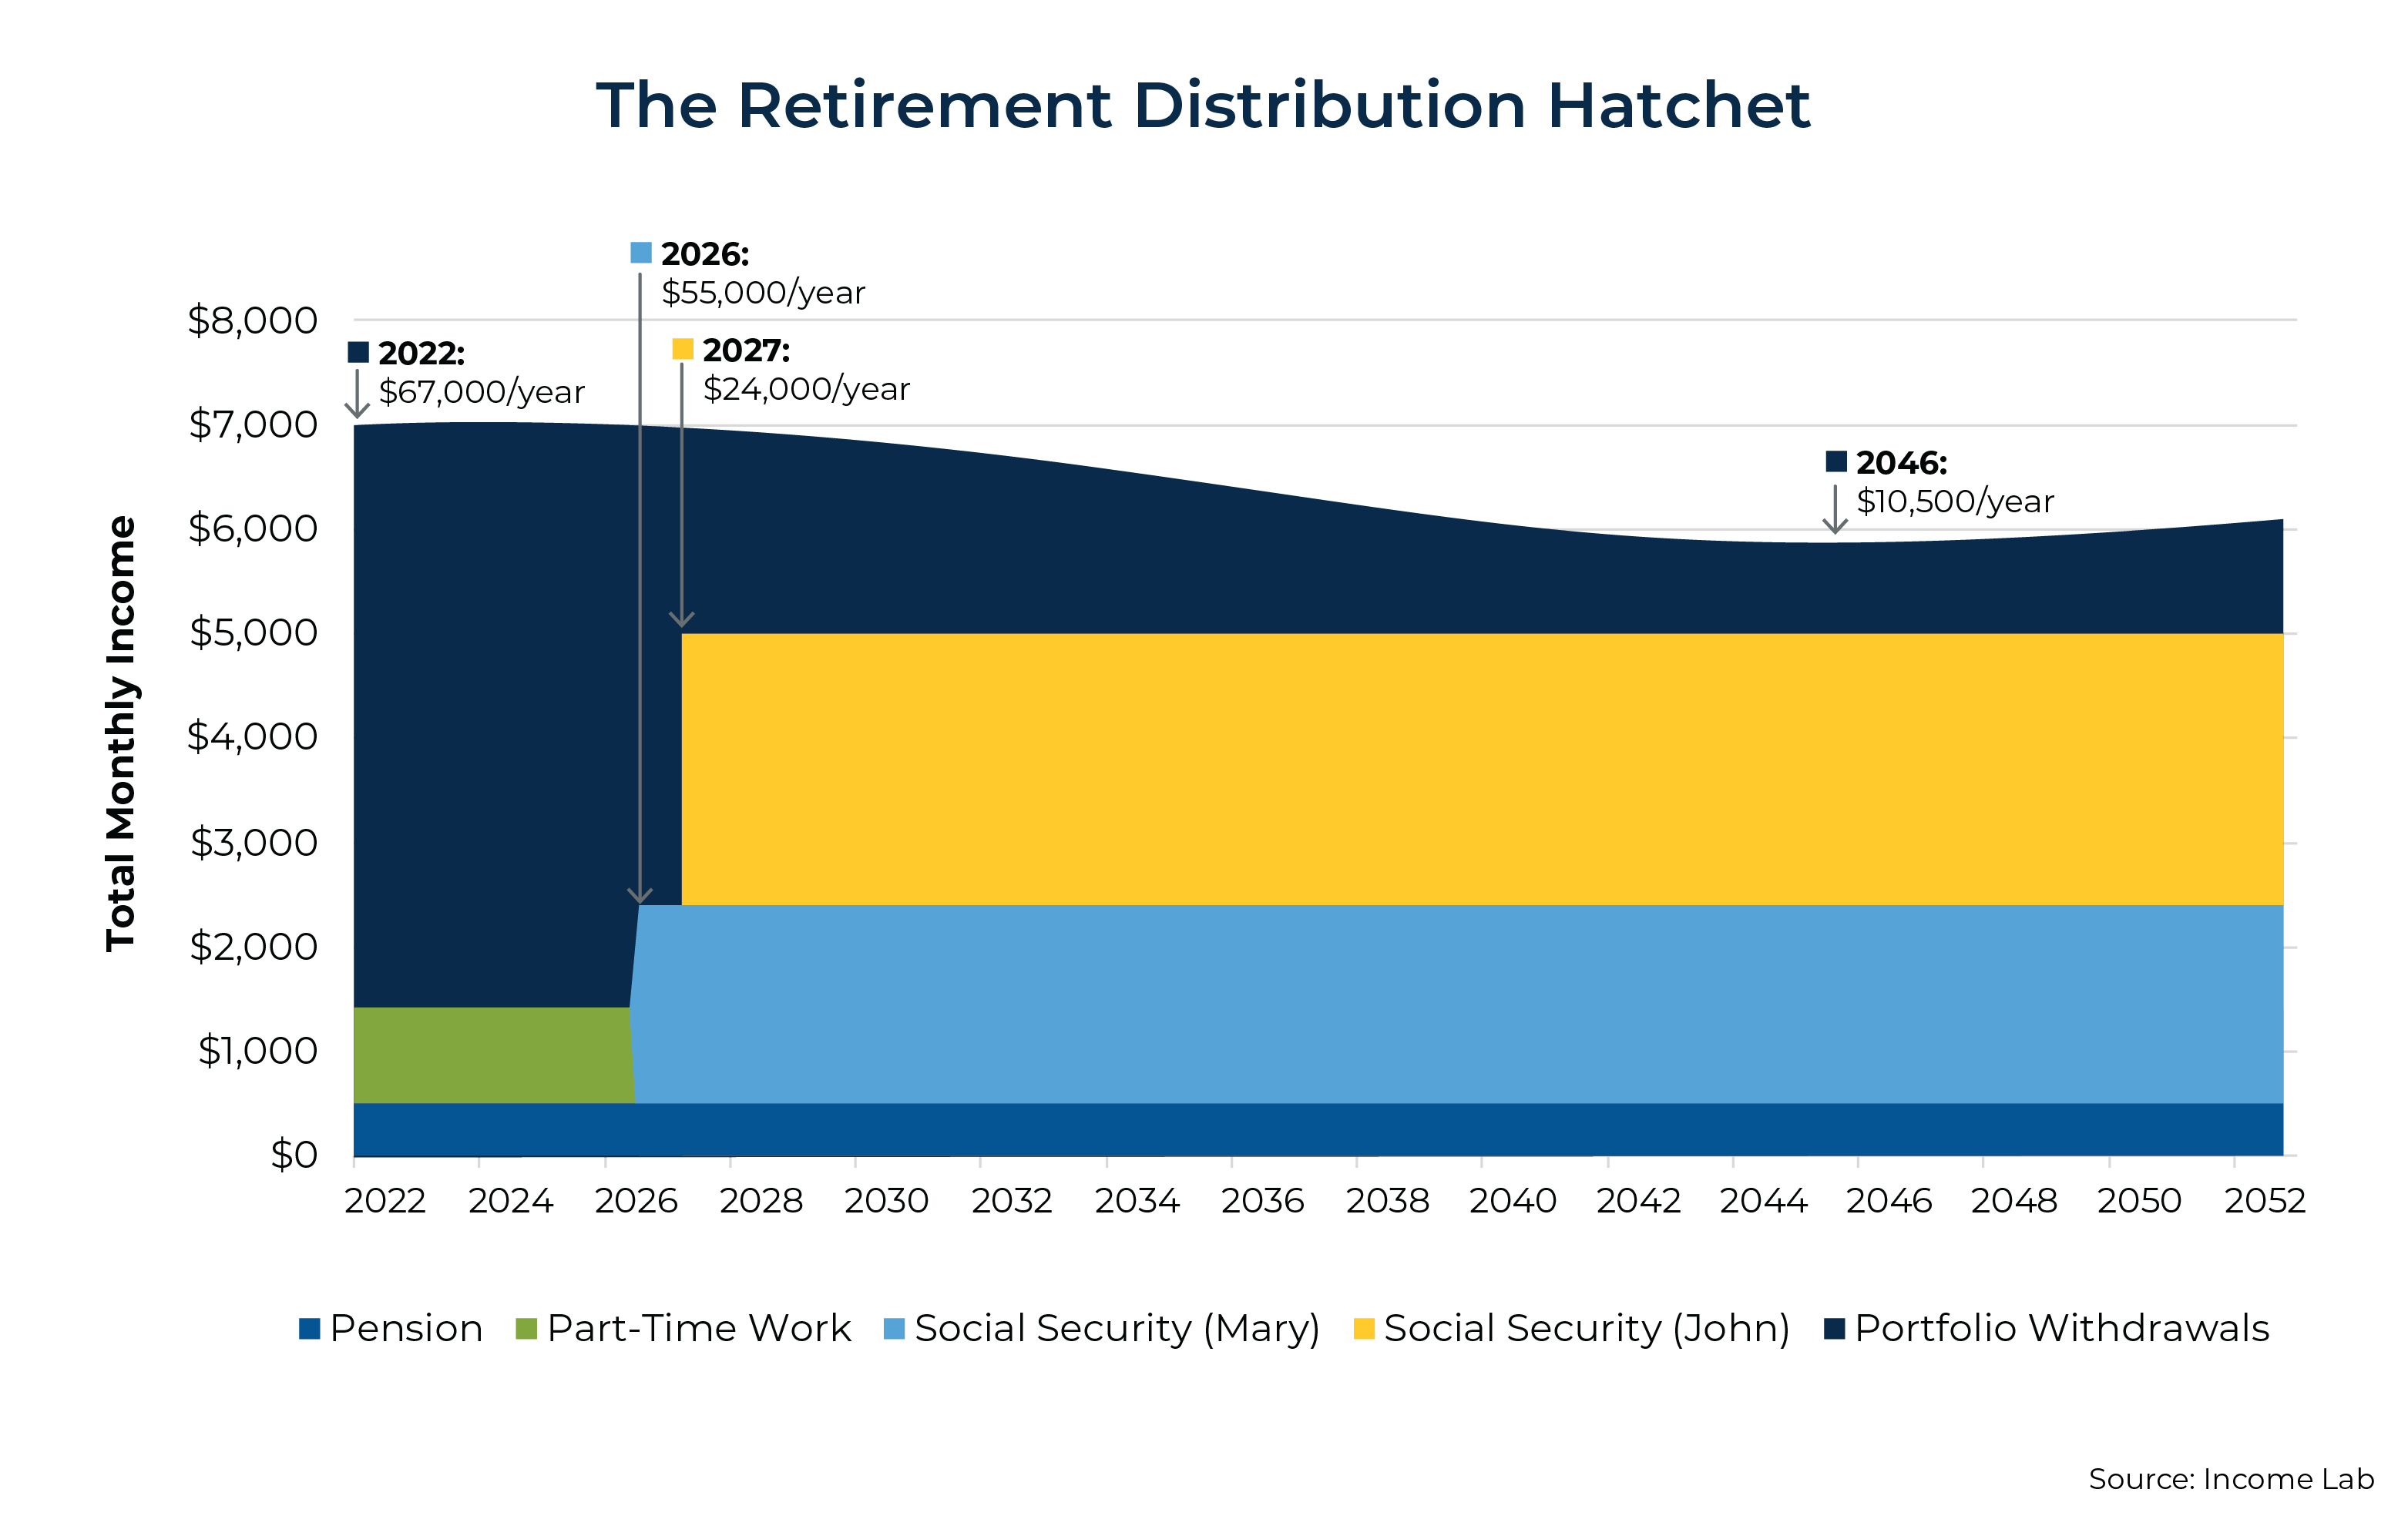
\includegraphics[width=\linewidth,height=0.48\textheight,keepaspectratio]{hatchet.png}
\end{center}
\vspace{2pt}

\newpage
% ================= PAGE 2: vertical Gantt =================
{\color{ink}\fontsize{16}{19}\selectfont\bfseries Retirement Account Timeline}\\[2pt]
{\color{graytext}\small Which accounts to draw from, receive income from, or act on for ages 50 to 90.}\\[8pt]

\begin{center}
\begin{tikzpicture}[font=\sffamily]

% lane centers
\def\la{1.0}\def\lb{2.9}\def\lc{4.8}\def\ld{6.7}\def\le{8.6}\def\lf{10.5}\def\lg{12.4}

% faint lane backgrounds
\foreach \x in {\la,\lb,\lc,\ld,\le,\lf,\lg}{
  \fill[lane] ({\x-0.72},\yy{50}) rectangle ({\x+0.72},\yy{90});}

% horizontal gridlines + age labels
\foreach \a in {50,55,60,65,70,75,80,85,90}{
  \draw[grid, line width=0.5pt] ({0.05},\yy{\a}) -- ({13.15},\yy{\a});
  \node[anchor=east, font=\footnotesize, text=graytext] at ({-0.05},\yy{\a}) {\a};}

% "AGE" axis marker with down arrow
\node[anchor=south east, font=\scriptsize\bfseries, text=graytext] at ({-0.05},0.05) {AGE};
\draw[graytext, line width=0.8pt, -{Stealth[length=4pt]}] ({-0.72},\yy{51}) -- ({-0.72},\yy{89});

% ---- bars ----
\barlane{\la}{50}{55}{drawA}                 % taxable bridge
\barlane{\lb}{55}{60}{drawB}                 % roth ladder
\barlane{\lc}{59.5}{90}{drawC}               % traditional / roth
\barlane{\ld}{50}{55}{amber}                 % conversions - build
\barlane{\ld}{65}{75}{amber}                 % conversions - cleanup
\barlane{\le}{55}{90}{penblue}               % pension
\barlane{\lf}{62}{90}{ssblue}                % social security
\barlane{\lg}{75}{90}{rust}                  % rmd

% small in-bar cues
\node[white, font=\tiny\bfseries, rotate=90] at ({\ld},\yy{52.5}) {BUILD};
\node[white, font=\tiny\bfseries, rotate=90] at ({\ld},\yy{70}) {CLEANUP};

% ---- lane headers ----
\lhead{\la}{Taxable}{bridge}{drawA}
\lhead{\lb}{Roth}{ladder}{drawB}
\lhead{\lc}{Traditional}{/ Roth}{drawC}
\lhead{\ld}{Roth}{conversions}{amber}
\lhead{\le}{Pension}{}{penblue}
\lhead{\lf}{Social}{Security}{ssblue}
\lhead{\lg}{RMDs}{}{rust}

% ---- milestones (right margin) ----
\event{50}{\textbf{50} \, Retire; roll both 401(k)s into a Traditional IRA}
\event{55}{\textbf{55} \, Pension starts; first Roth rung matures}
\event{59.5}{\textbf{59\textonehalf} \, All accounts unlock penalty-free}
\event{62}{\textbf{62} \, Social Security begins}
\event{65}{\textbf{65} \, Medicare; ACA ends; cleanup conversions begin}
\event{75}{\textbf{75} \, Required minimum withdrawals begin}

\end{tikzpicture}
\end{center}

\vspace{6pt}
% ---- legend ----
\begin{center}

\begin{tikzpicture}[font=\sffamily]
\foreach \c/\t [count=\i] in {drawB/{Spending draw}, amber/{Conversion (action you take)},
     ssblue/{Guaranteed income}, rust/{Required (forced) withdrawal}}{
  \pgfmathsetmacro\x{(\i-1)*4.35}
  \fill[\c, rounded corners=1.5pt] ({\x},0) rectangle ({\x+0.42},0.32);
  \node[anchor=west, font=\scriptsize, text=ink] at ({\x+0.55},0.16) {\t};}
\end{tikzpicture}
\end{center}

\end{document}